\documentclass{article}

\title{Square joy: tile crush}
\subtitle{Exploding tiles in J.}
\date{2024-12-16}
\modified{2024-12-16}

\keyword{j}
\keyword{arrays}
\keyword{puzzles}

\begin{document}

\section*

This article presents a solution to a programming puzzle using the \href{https://www.jsoftware.com/}{\textsc{j} programming language}.
The challenge is implementing mechanics for a tile-matching game using a data-parallel array-oriented approach (no stinking loops).

This article is not an introduction to the \textsc{j} programming language,
but it explains enough details to follow the solution even if you aren't familiar with the language.

\section{problem}{The problem: stabilize the game board}

Our game is a simplified version of the popular \href{https://en.wikipedia.org/wiki/Candy_Crush_Saga}{Candy Crash Saga} game:
\begin{enumerate}
\item A rectangular board contains square tiles of different types.
\item When three or more identical tiles appear next to one another in the same row or column, they explode and leave space.
\item Tiles experience gravity: they fall if there is space below them.
\item Moving tiles don't explode.
\item If there are multiple exploding sections, the explosions happen simultaneously.
\end{enumerate}

The goal is to implement the board update mechanics after the player makes a move.
The mechanics of the player moves are out of scope.

\section{board-representation}{The board representation}

I will represent the board as a numeric matrix.
Zero indicates an empty tile, and integers \math{1} through \math{K} correspond to tile types.

The board's columns will require more transformations than rows (gravity works column-wise),
so our board representation will be transposed compared to the user's view.
Matrix rows will correspond to columns in the interface and vice-versa.

I will use a nine-by-nine board with five tile types for all examples.

\begin{code}[j]
\emph{NB. The number of tiles types, including the empty zero tile.}
   K =. 6

\emph{NB. The board I will use for examples (your board may vary).}
\emph{NB. 9 9 \$ K creates a 9x9 board filled with integer K. }
\emph{NB. ?. 9 9 \$ K fills that board with random integers in range 0..K. }
   Board =. \href{https://code.jsoftware.com/wiki/Vocabulary/querydot}{?.} 9 9 \href{https://code.jsoftware.com/wiki/Vocabulary/dollar#dyadic}{\$} K
0 2 4 0 5 4 4 4 2
1 3 2 1 5 1 2 3 4
1 5 5 3 1 1 0 4 3
2 4 3 5 0 4 3 5 5
0 1 2 0 4 5 3 5 5
0 3 4 4 0 4 3 1 0
0 0 1 5 1 2 4 0 4
3 2 4 4 4 1 3 1 3
5 1 2 5 1 5 0 5 2
\end{code}

The numeric board is hard to look at, so let's write a function to visualize it using our \href{/posts/04-square-joy-trapped-rain-water.html#viewmat}{old friend}, \href{https://code.jsoftware.com/wiki/Studio/Viewmat}{viewmat}.

\begin{code}[j]
   require 'viewmat'
   viewboard =. {{ (255 255 255 , 0 0 128 ,: 128 128 128) viewmat |: y }}
   viewboard Board
\end{code}

\begin{figure}
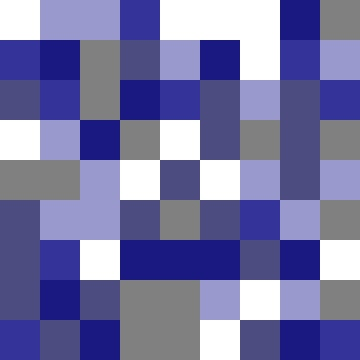
\includegraphics{/images/34-original-board.jpg}
\end{figure}

Ah, much better.
The whitespace corresponds to the space,
and different colors correspond to tile types.

Our tiles seem to float in the air; let's make them fall.

\section{gravity}{Implementing gravity}

The law of gravity requires heavy stuff to go down and light stuff to bubble.
In our board representation, the gravity pulls to the right,
so all the empty zero tiles must shift to the front of each row.
In the algorithm speak, we need a \href{https://en.cppreference.com/w/cpp/algorithm/stable_partition}{stable partition},
where the partition predicate is equality to zero.

\begin{code}
   \emph{NB. The first row before and after applying the stable partition.}
0 2 4 0 5 4 4 4 2
0 0 2 4 5 4 4 4 2
\end{code}

The simplest reincarnation of stable partition involves selecting matching and non-matching elements and gluing them together.
The \href{https://code.jsoftware.com/wiki/Vocabulary/number#dyadic}{copy} function (\code{#}) will help us select items given a boolean mask,
and \href{https://code.jsoftware.com/wiki/Vocabulary/comma#dyadic}{append} (\code{,}) will glue the results.

\begin{code}[j]
   \emph{NB. \{\{ and \}\} \href{https://code.jsoftware.com/wiki/Vocabulary/DirectDefinition}{define an anonymous function}}
   \emph{NB. where y is the implicitly defined right argument.}
   \emph{NB. We can also define the function tacitly as (#~ <:\&0),(#~ >\&0)"1}

   gravity =. {{ ((y=0)#y),(y~:0)#y }}"1
   gravity Board
0 0 2 4 5 4 4 4 2
1 3 2 1 5 1 2 3 4
0 1 5 5 3 1 1 4 3
0 2 4 3 5 4 3 5 5
0 0 1 2 4 5 3 5 5
0 0 0 3 4 4 4 3 1
0 0 0 1 5 1 2 4 4
3 2 4 4 4 1 3 1 3
0 5 1 2 5 1 5 5 2
   viewboard gravity Board
\end{code}

\begin{figure}
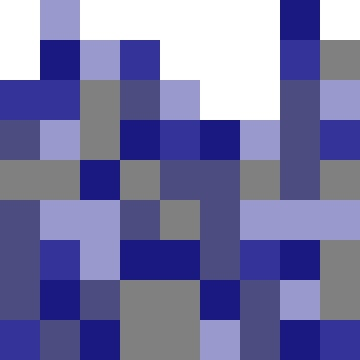
\includegraphics{/images/34-gravity-applied.jpg}
\end{figure}

The \code{"1} annotation tells the \textsc{j} interpreter that we intended the \code{gravity} function to work on one-dimensional arrays.
When we apply this function to a matrix, the interpreter automatically maps the function over each row.

Let's apply gravity to our example board to simplify further exploration.

\begin{code}[j]
   Board =. gravity Board
\end{code}

\section{matching-tiles}{Matching tiles}

We will first find tile matches in columns (rows of the board representation) and then extend the solution to work on both dimensions.

The core idea is to annotate each tile with the size of the longest run it's a member of.
Let's fix a specific row (the first board row) and the tile type (\code{4}) for now.

\begin{code}[j]
   R =. 0 0 2 4 5 4 4 4 2
\end{code}

Let's isolate the tiles we're focused on.

\begin{code}[j]
   R=4
0 0 0 1 0 1 1 1 0
\end{code}

Our life will be easy if we can replace each \code{1} with the length of the run in which this element appears.
For example, \code{0 0 0 1 0 1 1 1 0} should become \code{0 0 0 1 0 3 3 3 0}.

There are many ways to achieve this outcome; I will implement it in two passes over the boolean array.
In the first pass, we compute the running sum within each run, resetting the counter as soon as we hit zero.
In the second pass, we traverse the array backward and replace each item with the maximum within its run.

\begin{code}
0 0 0 1 0 1 1 1 0  \emph{NB. the original mask}
0 0 0 1 0 1 2 3 0  \emph{NB. sum items left-to-right within each run }
0 0 0 1 0 3 3 3 0  \emph{NB. max items right-to-left within each run }
\end{code}

The \href{https://code.jsoftware.com/wiki/Vocabulary/fcap}{fold} operator is a convenient tool to implement the first scan.
We will use its version that accepts three arguments: the initial accumulator value (\code{0}), the reduce function (\code{x * (x + y)}), and the post-processing step (the identity function, \href{https://code.jsoftware.com/wiki/Vocabulary/squarert}{same} \code{]}).

\begin{code}[j]
   S =. 0 ] F:. {{x*x+y}} R=4
   S
0 0 0 1 0 1 2 3 0
\end{code}

The second scan requires a fold that traverses the sequence in reverse (\code{F::}).
This time, our reduce function takes the maximum of the accumulator and the current item unless the item is zero (\code{(x>0) * (x >. y)}).
Since reverse fold produces items backward, we must \href{https://code.jsoftware.com/wiki/Vocabulary/bardot}{reverse} (\code{|.}) its result to get the sequence we need.

\begin{code}[j]
   0 ] F:: {{(x>0)*x>.y}} S
0 3 3 3 0 1 0 0 0

   |. 0 ] F:: {{(x>0)*x>.y}} S
0 0 0 1 0 3 3 3 0
\end{code}

Let's capture our progress in the \code{runs} function.

\begin{code}[j]
   NB. Given a bool mask, compute the longest run for each item.
   NB. [*+ is a shorter way to write {{x*(x+y)}}.

   runs =. {{ |. 0 ] F:: {{ (x>0) * x>.y }} 0 ] F:. ([*+) y }}"1
\end{code}

We solved the problem for a single tile type in a single row.
We must extend our solution to handle each row, column, and tile type.
\textsc{j} gives us per-row application for free thanks to the \code{runs} \href{https://code.jsoftware.com/wiki/Vocabulary/quote}{rank specification} (\code{"1}):

\begin{code}[j]
   runs Board=4
0 0 0 1 0 3 3 3 0
0 0 0 0 0 0 0 0 1
0 0 0 0 0 0 0 1 0
0 0 1 0 0 1 0 0 0
0 0 0 0 1 0 0 0 0
0 0 0 0 3 3 3 0 0
0 0 0 0 0 0 0 2 2
0 0 3 3 3 0 0 0 0
0 0 0 0 0 0 0 0 0
\end{code}

We handle columns by running \code{runs} on a transposed board and transposing the result.

\begin{code}[j]
   |: runs |: Board=4
0 0 0 1 0 1 1 1 0
0 0 0 0 0 0 0 0 1
0 0 0 0 0 0 0 1 0
0 0 1 0 0 1 0 0 0
0 0 0 0 2 0 0 0 0
0 0 0 0 2 1 1 0 0
0 0 0 0 0 0 0 1 1
0 0 1 1 1 0 0 0 0
0 0 0 0 0 0 0 0 0
\end{code}

\mathml{\mi{transpose} \mo{\circ} \mi{f} \mo{\circ} \mi{transpose}} is a special case of the \mathml{\msup{\mi{g}}{\mn{-1}} \mo{\circ} \mi{f} \mo{\circ} \mi{g}} pattern\sidenote{sn-self-inverse}{
  Transposition is an \href{https://en.wikipedia.org/wiki/Involution_(mathematics)}{involution}: it undoes itself.
}
that's so ubiquitous in mathematics that \textsc{j} defines a convenient operator to express it: \href{https://code.jsoftware.com/wiki/Vocabulary/ampdot}{under} (\code{\&.}).

\begin{code}[j]
   runs &. |: Board=4
0 0 0 1 0 1 1 1 0
0 0 0 0 0 0 0 0 1
0 0 0 0 0 0 0 1 0
0 0 1 0 0 1 0 0 0
0 0 0 0 2 0 0 0 0
0 0 0 0 2 1 1 0 0
0 0 0 0 0 0 0 1 1
0 0 1 1 1 0 0 0 0
0 0 0 0 0 0 0 0 0
\end{code}

We can package the row-wise and column-wise transformations into a single function by taking the maximum of their outputs.

\begin{code}[j]
   ((runs &. |:) >. runs) Board=4
0 0 0 1 0 3 3 3 0
0 0 0 0 0 0 0 0 1
0 0 0 0 0 0 0 1 0
0 0 1 0 0 1 0 0 0
0 0 0 0 2 0 0 0 0
0 0 0 0 3 3 3 0 0
0 0 0 0 0 0 0 2 2
0 0 3 3 3 0 0 0 0
0 0 0 0 0 0 0 0 0
\end{code}

To extend the solution to all tile types (not just \code{4}), we generate the list of non-zero tiles (\code{\}. i. K}),
match the board against every type, producing a list of disjoint boolean matrices (\code{Board ="_ 0 \}. i. K}),
compute runs for each matrix,
and sum the results.

\begin{code}[j]
   +/ ((runs &. |:) >. runs)"2 Board ="_ 0 \}. i. K
0 0 2 1 2 3 3 3 1
1 1 2 1 2 2 1 1 1
0 1 2 2 1 2 2 1 1
0 1 1 1 1 1 2 2 2
0 0 1 1 2 1 2 2 2
0 0 0 1 3 3 3 1 1
0 0 0 1 1 3 1 2 2
1 1 3 3 3 3 1 1 1
0 1 1 1 1 3 2 2 1
\end{code}

Comparing the result with the explosion threshold gives us the mask of tiles eligible for explosion.

\begin{code}[j]
   3 <: +/ ((runs &. |:) >. runs)"2 Board ="_ 0 \}. i. K
0 0 0 0 0 1 1 1 0
0 0 0 0 0 0 0 0 0
0 0 0 0 0 0 0 0 0
0 0 0 0 0 0 0 0 0
0 0 0 0 0 0 0 0 0
0 0 0 0 1 1 1 0 0
0 0 0 0 0 1 0 0 0
0 0 1 1 1 1 0 0 0
0 0 0 0 0 1 0 0 0
\end{code}

\begin{figure}
\marginnote{sn-explosion-mask}{
  Side by side: the board before the explosion (left) and the mask of tiles eligible for explosion (right).
}
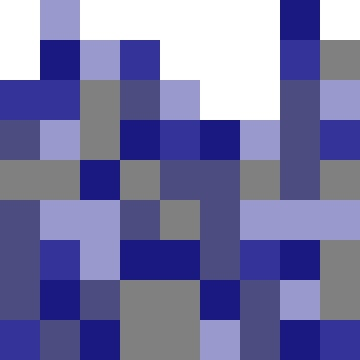
\includegraphics{/images/34-gravity-applied.jpg}
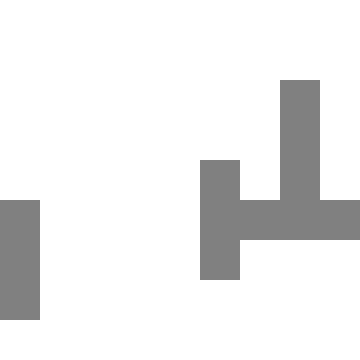
\includegraphics{/images/34-explosion-mask.jpg}
\end{figure}

One last annoyance is that our expression depends on the constant \code{K}.
We can make it less context-dependent by computing the set of unique positive tile types on the board.
The \href{https://code.jsoftware.com/wiki/Vocabulary/tildedot}{nub} (\code{~.}) and \href{https://code.jsoftware.com/wiki/Vocabulary/comma}{ravel} (\code{,}) verbs make it easy.

\begin{code}[j]
   \emph{NB. compute the set of unique tiles on the board.}
   ~.,Board
0 2 4 5 1 3

   \emph{NB. leave only positive values.}
   (#~ >&0) ~.,Board
2 4 5 1 3

   \emph{NB. update the tile matching expression to use the tile types from the board.}
   3 <: +/ ((runs &. |:) >. runs)"2 Board ="_ 0 (#~ >&0) ~., Board
0 0 0 0 0 1 1 1 0
0 0 0 0 0 0 0 0 0
0 0 0 0 0 0 0 0 0
0 0 0 0 0 0 0 0 0
0 0 0 0 0 0 0 0 0
0 0 0 0 1 1 1 0 0
0 0 0 0 0 1 0 0 0
0 0 1 1 1 1 0 0 0
0 0 0 0 0 1 0 0 0
\end{code}

\section{putting-together}{Putting it all together}

It's time to combine the gravity and tile matching into the board update function.
This function should find matching tiles, ``explode'' them by replacing these tiles with zero tiles, and apply gravity.

The expression from the previous section gives us a mask of all the tiles we need to explode.
We implement the explosion by multiplying the board by the inverse of that mask.

\begin{code}[j]
   explode =. {{ y * 2>: +/ ((runs &. |:) >. runs)"2 y ="_ 0 (#~ >&0) ~., y }}
   viewboard explode Board
\end{code}

\begin{figure}
\marginnote{sn-board-after-explosion}{
  Side by side: the board before and after tile explosion.
}
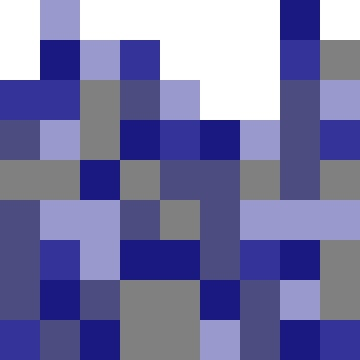
\includegraphics{/images/34-gravity-applied.jpg}
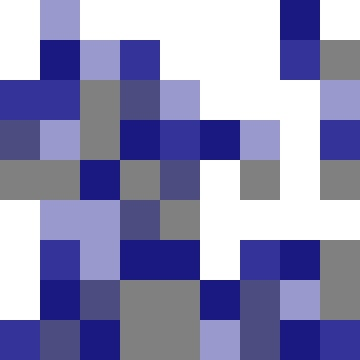
\includegraphics{/images/34-exploded-board.jpg}
\end{figure}

Let's see what happens when we add gravity.
\begin{figure}
\marginnote{sn-explosion-gravity}{
  Side by side: the board right after tile explosion and after the gravity action.
}
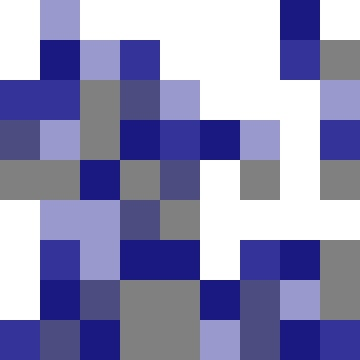
\includegraphics{/images/34-exploded-board.jpg}
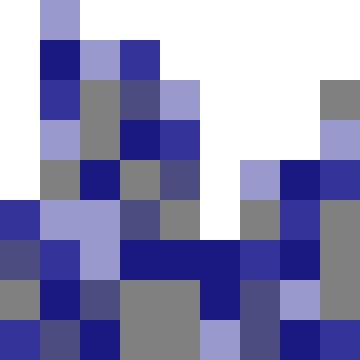
\includegraphics{/images/34-exploded-gravity-board.jpg}
\end{figure}

Look, there are more tiles to explode now!
We shall keep updating the board until it stops changing.
Luckily, \textsc{j} gives us a perfect operator for that: \href{https://code.jsoftware.com/wiki/Vocabulary/hatco#u.5E:_.28Converge.29}{converge} (\code{^:_})\sidenote{sn-converge-chicken}{
  The \code{^:_} glyph reminds me of a curious chicken lying on the grass and looking at the infinite sky.
}. We compose gravity and tile explosion using the \href{https://code.jsoftware.com/wiki/Vocabulary/atco}{at} operator (\code{@:})

\begin{code}[j]
   update =. (explode @: gravity) ^:_

   viewboard update Board
\end{code}

\begin{figure}
\marginnote{sn-full-update}{
  Side by side: the example board after the gravity applied and the stabilized final board.
}
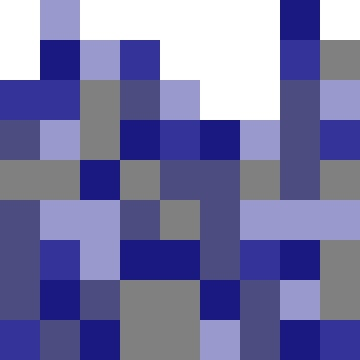
\includegraphics{/images/34-gravity-applied.jpg}
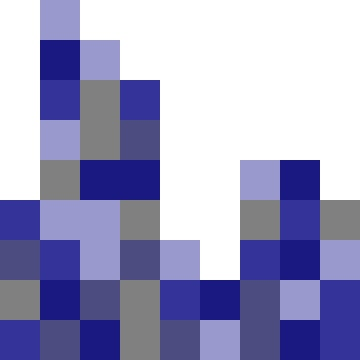
\includegraphics{/images/34-board-final.jpg}
\end{figure}

Before we close, let's see what happens when we imitate the player's move by swapping two tiles (the fifth row, the second, and the third columns).

\begin{code}
   \emph{NB. swaps items in the right arg according to the spec in the left arg.}
   swap =. {{ (|. x { y) x } y }}

   viewboard (1 4; 2 4) swap update Board
   viewboard update (1 4; 2 4) swap update Board
\end{code}

\begin{figure}
\marginnote{sn-after-swap}{
  Side by side: the stabilized board with two tiles swapped and the updated board after the move.
}
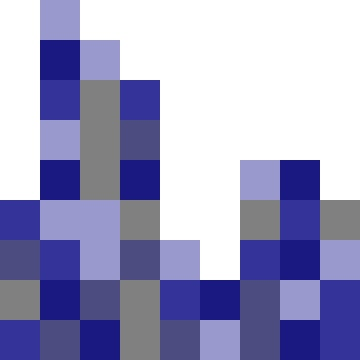
\includegraphics{/images/34-swap-tiles.jpg}
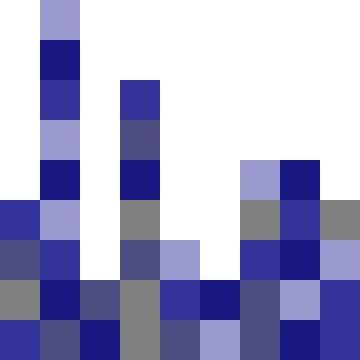
\includegraphics{/images/34-update-after-swap.jpg}
\end{figure}

That's it!
We implemented the core game mechanics with only four lines of code:

\begin{code}[j]
gravity =. {{ ((y=0)#y),(y~:0)#y }}"1
runs    =. {{ |. 0 ] F:: {{ (x>0) * x>.y }} 0 ] F:. ([*+) y }}"1
explode =. {{ y * 2 >: +/ ((runs &. |:) >. runs)"2 y ="_ 0 (#~ >&0) ~., y }}
update  =. (explode @: gravity) ^:_
\end{code}

\section{exercises}{Exercises}

If you enjoyed the puzzle and want to spend more time with it,
here are a few suggestions on how to keep the fun going:

\begin{itemize}
\item Add support for non-rectangular boards.
\details{Hint}{
  Add a new tile type that doesn't explode or move (I'd use \code{_1} to indicate this tile on the board).
  When applying gravity to a column, \href{https://code.jsoftware.com/wiki/Help/Primer/090_Cut_;.}{cut} it into subarrays using the new tile type as a fret.
  Apply the gravity rules to each subarray, then join them.
}

\item Add horizontal gravity.
If an explosion creates empty columns, let the non-empty columns gather.
\details{Hint}{
  Replace empty columns with a new tile type (e.g., \code{_2}).
  Apply the gravity to the transposed board using this new tile type as the space indicator.
  The exact partitioning rules depend on the variation of gravity you want to implement.
}
\end{itemize}

\end{document}
